\documentclass[nogrid]{MBE}%


\usepackage{url}

\jshort{mst}

\volname{}

\jvolume{0}

\jvol{}

\jissue{0}

\pubyear{2019}

\mstype{Article}

\artid{012}

\begin{document}

\title{Mode and tempo of promoter evolution in the Paramecium aurelia species complex}


\author[Raborn et al.]{R. Taylor \surname{Raborn},$^{\ast,1,2}$ Timothy Licknack,$^{1,2}$ Wanfeng Guo,$^{1,2}$ Shannon N. Snyder,$^{1,2}$ and Michael Lynch$^{1,2}$}

\address{$^{1}$Biodesign Center for Mechanisms of Evolution\\
$^{2}$School of Life Sciences\\
Arizona State University, Room C445 797 E. Tyler Street, Tempe, AZ 85281}


%\history{Received xx xxxxx 2019; reviews returned xx xxxx 2019; accepted xx xxxxx 2019}

\coresp{E-mail: rtraborn@asu.edu}

%\datade{The POPRES data were obtained from dbGaP (accession no. phs000145.v1.p1).}

\abstract{Goes here
}

\keyword{cis-regulatory regions, Paramecium, promoter evolution, TSS profiling.}

\maketitle



\section{{Introduction}\label{sec:Intro}}

Enter introduction here



\section{Demographic structure}

More words here

\subsection{Subsection 1}



\subsubsection{Subsection 2}




\paragraph{Paragraph header} 



\begin{arabiclist}
\item Item 1

\item Item 2

\item Item 3
\end{arabiclist}

\begin{itemize}
\item Consider a fall in population induced by a decline in the number of births in the economy,
taking as given mortality and migration.

\item It is well known that a lower population growth raises the capital--labor ratio in the Solow--Swan
growth model.

\item The same property holds in Diamond's (1965) overlapping generations model, and it enhances welfare
as long as the economy is dynamically efficient; i.e., when the interest rate exceeds the
population growth rate.
\end{itemize}
 A similar trend is observed in the United
States and advanced European countries (Gustafsson and Kalwij, 2006), and also in Canada,
Australia, and New Zealand (Sardon, 2006). Interestingly, as pointed out by Bongaarts and Feeney
(1998), even when the cohort's lifetime fertility rate (the number of children a mother has in her
lifetime) does not fall, the delayed childbearing alone leads to a decline in the number of
childbirths, measured by the total period fertility rates (TPFRs). %Ogawa and Retherford (1993),
%Kohler et al. (2002), and Sobotka (2004) confirmed that, to a certain extent, the delay of
%marriage and motherhood is responsible for the observed period fertility rate decline (now known
%as the `tempo effect').


\section{Model\label{sec:Model}}

\subsection{Demographic structure}



i.e.:
\begin{equation}
\lambda_{t}=\left\{
\begin{array}
[c]{cc}%
0, & t<0,\\
\lambda, & t\geq0.
\end{array}
\right.  \label{eq:lambda}%
\end{equation}


\begin{figure}[t]
\begin{center}
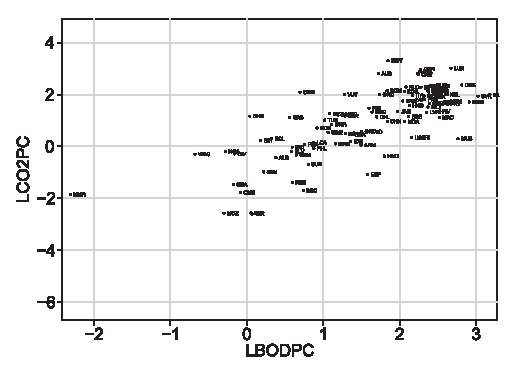
\includegraphics[height=0.21\textheight]{flrf1.eps}
\end{center}
\caption{Fluctuations in Cohort Size $N_{t}$ over Generations.}%
\label{fig:popdynamics}%
\end{figure}

%\TWOfig{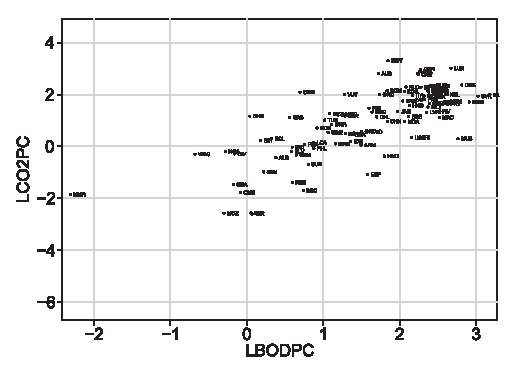
\includegraphics[width=10pc]{flrf1.eps}}{Fluctuations in
%Cohort Size $N_{t}$ over
%Generations.\label{fig:popdynamics}}{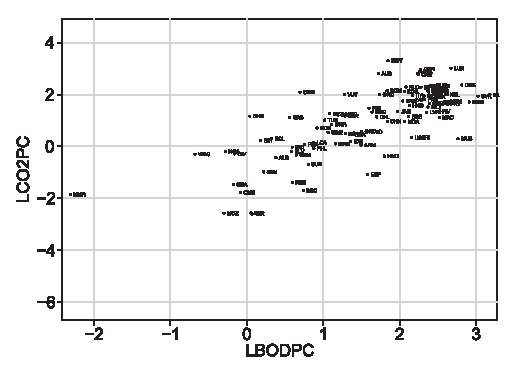
\includegraphics[width=10pc]{flrf1.eps}}{Dynamics
%of Labor Force $L_{t}$.\newline
%\phantom{\hskip5pc}\label{fig:labordynamics}}

where $C$ is a constant term defined as $C\equiv\beta\log\beta-(1+\beta
)\log(1+\beta)+\beta\log A\alpha+(1+\beta)\log A\left(  1-\alpha\right)  $.
Similarly, long-term welfare in the benchmark economy ($\lambda=0$) can be
written as:
\begin{equation}
U^{\ast}=\left(  1+\beta\right)  \log[A\alpha\left(  k^{\ast}\right)
^{2\alpha-1}+\left(  k^{\ast}\right)  ^{\alpha}]-\beta\left(  1-\alpha\right)
\log k^{\ast}+C. \label{eq:U_benchmark}%
\end{equation}

\begin{table}[!t]%1
\tableparts{\caption{SH test results on nuclear and mitochondrial phylogenetic trees}\label{tab1}}
{\begin{tabular*}{\columnwidth}{@{\extracolsep{\fill}}lld{6,0}d{6,0}@{}}\toprule Sequence data &
\mcc{Tree} & \mcc{$-\ln~L$} & \mcc{SH test $P$-value} \\\colrule mtDNA& mtDNA& -109219.5& 0.5 \\
[0.1pt]
mtDNA& Nuclear& -61720.8& \mcc{\hspace*{5pt}$<{0.00001}$} \\
Nuclear& mtDNA& -113033.1& \mcc{\hspace*{5pt}$<{0.00001}$} \\
Nuclear& Nuclear& -60699.9& 0.5 \\\botrule
\end{tabular*}}
{}
\end{table}

%
\section{Supplementary Material}
Supplementary tables S1?S7 and figures S1?S11 are available  at Molecular Biology and Evolution
online (http://www.mbe.oxfordjournals.org/).

\section{Acknowledgments}

The authors gratefully acknowledge the help of Robert Policastro and Gabriel Zentner at Indiana University Bloomington for technical assistance and use of laboratory facilities.


\bibliographystyle{natbib}%%%%natbib.sty
\bibliography{refs}%%%refs.bib

\end{document}